\section{Getting Help}

Learn how to make good use of the Help files. Often you will find useful examples at the bottom of each Help page. Be sure to scroll down to check them out, even (or specially) if you don't fully understand the text explanations at first. You can run the examples directly from the Help browser, or you can copy and paste the code onto a new window to play around with it. 

Select any valid class or method in your SuperCollider code (double-clicking the word will select it), and hit [ctrl+D] to open the corresponding Help file. If you select a class name (for example, \texttt{MouseX}), you will be directed to the class Help file. If you select a method, you will be directed to a list of classes that understand that method (for example, ask for help on the method \texttt{scramble}).\footnote{Attention: SuperCollider will display in blue any word that starts with a Capital letter. This means that the color blue \emph{does not guarantee} that the word is typo-free: for example, if you type Sinosc (with wrong lowercase "o"), it will still show up in blue.}

Other ways to explore the Help files in the SuperCollider IDE are the ``Browse'' and ``Search'' links. Use Browse to navigate the files by categories, and Search to look for words in all Help files. Important note about the Help Browser in the SuperCollider IDE:
\begin{itemize}
\item Use the top-right field (where it says ``Find...'') to look for specific words \emph{within the currently open Help file} (like you would do a ``find'' on a website);
\item Use the ``Search'' link (to the right of ``Browse'') to search text \emph{across all Help files}.
\end{itemize}

When you first open parentheses to add arguments to a given method, SC displays a little ``tooltip help'' to show you what the expected arguments are. For example, type the beginning of line that you see in figure \ref{fig:tooltip}. Right after opening the first parenthesis, you see the tooltip showing that the arguments to a \texttt{SinOsc.ar} are \texttt{freq}, \texttt{phase}, \texttt{mul}, and \texttt{add}. It also shows us what the default values are. This is exactly the same information you would get from the \texttt{SinOsc} Help file. If the tooltip has disappeared, you can bring it back with [ctrl+Shift+Space].

\begin{figure}[h]
\centerline{\framebox{
	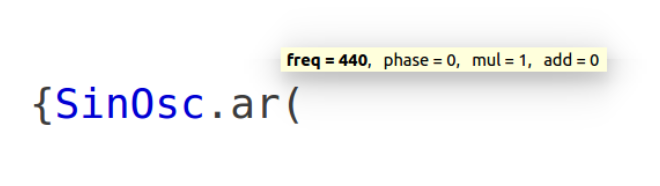
\includegraphics[scale=0.3]{fig-help-tooltip-crop.png}}}
\caption{Helpful info is displayed as you type.}
\label{fig:tooltip}
\end{figure}

Another shortcut: if you would like to explicitly name your arguments (like \texttt{SinOsc.ar(freq: 890)}), try hitting the tab key right after opening the parentheses. SC will autocomplete the correct argument name for you, in order, as you type (hit tab after the comma for subsequent argument names).

\bigskip
\todo[inline, color=green!40]{ 
TIP: Create a folder with your own ``personalized help files.'' Whenever you figure out some new trick or learn a new object, write a simple example with explanations in your own words, and save it for the future. It may come in handy a month or a year from now. 
}
\bigskip

The exact same Help files can also be found online at \url{http://doc.sccode.org/}.